\documentclass[../../main.tex]{subfiles}
\begin{document}

{\bf [解]}
対称性から下図の $\triangle OAB$ 内で $P$ がうごく時のみを考える．

\begin{figure}[htb]
\begin{center}
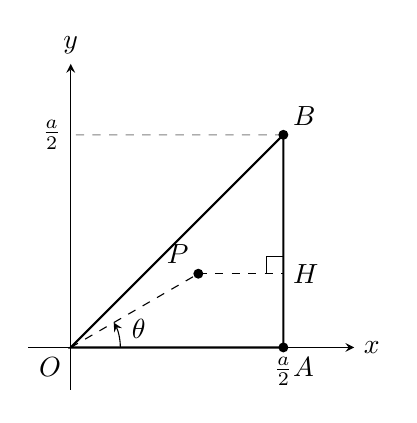
\begin{tikzpicture}[scale=1.8, >=stealth]
  % 1. 座標軸
  \draw[->] (-0.3,0) -- (2.0,0) node[right] {$x$};
  \draw[->] (0,-0.3) -- (0,2.0) node[above] {$y$};
  \node[below left] at (0,0) {$O$};

  % 2. 主要な点の座標定義 (a/2 = 1.5 とする)
  \coordinate (O) at (0,0);
  \coordinate (A) at (1.5,0);
  \coordinate (B) at (1.5,1.5);
  \coordinate (P) at (0.9,0.52); % r = 0.75/(1+cos(theta))
  \coordinate (H) at (1.5,0.52);

  % 3. 三角形 OAB の描画
  \draw[thick] (O) -- (A) -- (B) -- cycle;

  % 4. 補助線と目盛り (a/2)
  \draw[dashed, gray] (B) -- (0,1.5);
  \node[below] at (A) {$\frac{a}{2}$};
  \node[left] at (0,1.5) {$\frac{a}{2}$};

  % 5. 点 P, H 関連の描画
  \draw[dashed] (O) -- (P);
  \draw[dashed] (P) -- (H);
  
  % 直角マーク (Hにおける垂直記号)
  \draw (1.38, 0.52) -- (1.38, 0.64) -- (1.5, 0.64);

  % 6. 各点のプロットとラベル
  \fill (A) circle (1pt) node[below right] {$A$};
  \fill (B) circle (1pt) node[above right] {$B$};
  \fill (P) circle (1pt) node[above left] {$P$};
  \node[right] at (H) {$H$};

  % 7. 偏角 theta
  \draw[->] (0.35,0) arc (0:30:0.35);
  \node at (0.48,0.13) {$\theta$};

\end{tikzpicture}
\end{center}
\caption{点$P$の軌跡と$\triangle OAB$の関係}
\end{figure}

この時 $P$ と最も近い辺は $AB$ である．そこで $P$ から $AB$ に下ろした垂足を $H$ とし，$O$ を極，$x$軸正方向を始線とする極座標で $P(r,\theta)$ とおく（$r,\theta\ge 0$）．題意から，
\begin{align}
 \overline{OP}=\overline{PH} \\
\iff r=\frac{a}{2}-r\cos\theta \\
\iff r=\frac{\frac12 a}{1+\cos\theta} \quad (0\le\theta\le\pi/4) \label{eq:1}
\end{align}
となる．この時たしかに $P$ は $\triangle OAB$ 内にある．

以下面積を求める．対称性からもとめる面積 $S$，$S$ のうち $\triangle OAB$ 内のものを $S'$ として，
\begin{align}
S=8S' \label{eq:2}
\end{align}
である．具体的に$S'$を計算すると\cref{eq:1}から
\begin{align}
S'
  & =\int_0^{\pi/4}\frac{1}{2}r^2d\theta \\
  &= \frac{a^2}{8}\int_0^{\pi/4}\frac{1}{(1+\cos\theta)^2}d\theta \\
  &= \frac{a^2}{8}\int_0^{\pi/4}\frac{1}{4\cos^4\frac\theta2}d\theta \\
\end{align}
である．以下簡単のため $c=\cos\dfrac{\theta}{2},\ t=\tan\dfrac{\theta}{2}$ とすると
\begin{align}
S'
  & =\frac{a^2}{32}\int_0^{\pi/4}(1+t^2)\frac{1}{C^2}d\theta \\
  & = \frac{2a^2}{32}\left[t+\frac13t^3\right]_0^{\pi/4} \\
  &= \frac{a^2}{16}\left(\tan\frac\pi8+\frac13\tan^3\frac\pi8\right) \label{eq:3}
\end{align}
である．ここで$\tan\dfrac{\pi}{8}$について半角公式より
\begin{align}
 \tan\dfrac{\pi}{8} = \sqrt{\dfrac{1-\cos\dfrac{\pi}{4}}{1+\cos\dfrac{\pi}{4}}} = \sqrt{\dfrac{2-\sqrt{2}}{2+\sqrt{2}}} = -1 + \sqrt{2}
\end{align}
だから\cref{eq:3}に代入して
\begin{align}
S'
 & =\frac{a^2}{16}(-1+\sqrt2)\left(1+\frac13(-1+\sqrt2)^2\right) \\
 &= \frac{a^2}{16}(-1+\sqrt2)\left(\frac{6-2\sqrt2}{3}\right) 
\end{align}
となって，\cref{eq:2}に代入して
\begin{align}
S
  &=\frac{a^2}{2}\cdot\frac23(-1+\sqrt2)(3-\sqrt2) \\
  &= \frac{a^2}{3}(-5+4\sqrt2)
\end{align}
である．

\medskip
\noindent\textbf{[解2]}

\cref{eq:1}の方程式が放物線のものであることに気づけば，通常の座標系に映ることでより簡単に計算できる．
$P$ の軌跡は，$O$ を焦点，$AB$ を準線とする放物線で，その方程式は $\alpha=\dfrac{1}{4} a$ として
\begin{align}
y^2
  &=-4\alpha\left(x-\frac{a}{4}\right)\\
  &=-a\left(x-\frac a4\right)
\end{align}
である．

\begin{figure}[htb]
\begin{center}
\begin{tikzpicture}[scale=2, >=stealth]
  % パラメータ設定 (a/4 = 0.8 とする)
  % 放物線: x = -1/a * y^2 + a/4 = -0.3125 * y^2 + 0.8
  % 交点: y = (sqrt(2)-1)/2 * a ≒ 0.207 * 3.2 ≒ 0.663
  \def\aFour{0.8}
  \def\yIntersect{0.663}

  % 1. 領域 S' の斜線塗りつぶし
  % 0 <= y <= yIntersect において、x = y から x = -y^2/(4*aFour) + aFour まで
  \begin{scope}
    \fill[pattern=north east lines, pattern color=gray!80]
      (0,0) -- plot[domain=0:\yIntersect, samples=50] ({-0.3125*\x*\x + \aFour}, \x)
      -- cycle;
  \end{scope}

  % 2. 座標軸
  \draw[->] (-1.0, 0) -- (2.0, 0) node[right] {$x$};
  \draw[->] (0, -1.0) -- (0, 1.8) node[above] {$y$};
  \node[below right] at (0,0) {$O$};

  % 3. 放物線 y^2 = -a(x - a/4) の描画
  \draw[thick, domain=-1.1:1.3, samples=100] plot ({-0.3125*\x*\x + \aFour}, \x);

  % 4. 直線 x = y の描画
  \draw[dashed, domain=-0.3:1.2] plot (\x, \x) node[above right] {$x = y$};

  % 5. 補助線と目盛り
  % 交点から y 軸への破線
  \draw[dashed] ({\yIntersect}, {\yIntersect}) -- (0, {\yIntersect});

  % 目盛りラベル
  \node[left, font=\small] at (0, {\yIntersect}) {$\frac{\sqrt{2}-1}{2}a$};
  \node[below right, font=\small] at (\aFour, 0) {$\frac{a}{4}$};
  \node[below, font=\small] at ({2*\aFour}, 0) {$\frac{a}{2}$};

  % 6. 点のプロット
  \fill (0,0) circle (1pt);
  \fill (\aFour, 0) circle (1pt);
  \fill ({2*\aFour}, 0) circle (1pt);
  \fill ({\yIntersect}, {\yIntersect}) circle (1pt);

\end{tikzpicture}
\end{center}
\caption{放物線 $y^2 = -a\left(x - \frac{a}{4}\right)$ と領域 $S'$}
\end{figure}

よって上図斜線部の面積 $S'$ は
\begin{align}
S'
 &=\int_0^{\frac{\sqrt2-1}{2}a}\left(-\frac1ay^2+\frac a4\right)dy-\frac12\left(\frac{\sqrt2-1}{2}a\right)^2 \\
 &=-\frac1{3a}\left(\frac{\sqrt2-1}{2}a\right)^3+\frac a4\cdot\frac{\sqrt2-1}{2}a-\frac18(3-2\sqrt2)a^2
\end{align}
と計算され，[解1] と同じく $S=\dfrac{a^2}{3}(-5+4\sqrt2)$ を得る．


\newpage

\end{document}
